
\documentclass[paper=a4
               ,12pt
               ,DIV=12
               ,parskip=half
               ,titlepage=on
               ,headinclude 
               ,footinclude
               %,headtopline        % Oberlinie �ber dem Kopf
               ,headsepline
               ,footsepline         % Linie unter der Kopfzeile
               ,ilines 
                %,bibtotocnumbered                           
               ]{scrartcl}
              
\usepackage[english]{babel}              % Sprachanpassungen in Klassenoptionen [english, ngerman]
\usepackage[utf8]{inputenc}   % Zeicheneingabe per Tastatur (Umlaute, etc.)
\usepackage{csquotes}           % Anf�hrungszeichen sprachenabh�ngig \enquote{}
\usepackage[T1]{fontenc}        % Schriftencoding f�r das Dokument
\usepackage{lmodern, microtype} % Bessere Trennung und Absatzkontrolle
%\usepackage[pdftex]{graphicx}   % Einbindung von Graphiken in den Formaten .pdf, .jpg, .eps
\usepackage{enumerate}
\usepackage{wrapfig}  					% Tabelle von Text umfließen lassen   
          % Grafiken von Text umfließen lassen      
\usepackage{graphicx}	
\usepackage{blindtext,              % Blindtext erzeugen
            graphicx,               % Einbinden von Graphiken (.jpg, .pdf)
            amsmath,                % Mathematikpaket
            makeidx,                % Paket f�r das Stichwortverzeichnis
            booktabs,               % Tabellenlayout-Paket
            scrpage2,
            multicol,
            pifont,
            amssymb,
            array,
            amsfonts,
            tikz,
            longtable,
            multirow,
            sidecap,
            rotating
}
% \makeatletter
%\renewcommand{\ALG@name}{Algorithmus}
%\renewcommand{\listalgorithmname}{List of \ALG@name s}
% \makeatother

\newcommand{\sign}{\text{sign}} % Signum Zeichen

 \usepackage{setspace} % Zeilenabstände definieren mit \singlespacing, \onehalfspacing          

            
\makeindex

\usepackage[
    top=3cm,
    bottom=3.5cm,
    left=2.5cm,
    right=2.5cm
    ]
    {geometry}
\linespread{1.5}

\usepackage[normalem]{ulem}

\usepackage{array}

\usepackage{hyperref}

\usepackage{tabularx}  % for 'tabularx' environment and 'X' column type
\usepackage{ragged2e}  % for '\RaggedRight' macro (allows hyphenation)
\newcolumntype{Y}{>{\RaggedRight\arraybackslash}X} 
\usepackage{booktabs}
\usepackage{color}
\usepackage{tikz}
\usetikzlibrary{shapes,arrows}

%\usepackage[pdftex,colorlinks=true,backref]{hyperref}

%\usepackage{url}

\newcommand*{\quo}[1]{{\glqq #1\grqq}}
\newcommand{\argmax}[1]{\underset{#1}{\operatorname{arg}\,\operatorname{max}}\;}
\newcommand{\argmin}[1]{\underset{#1}{\operatorname{arg}\,\operatorname{min}}\;}

\usepackage[%                       % f�r nat-Stile laden, damit \citep und \citet verf�gbar sind
           round,                  % default f�r Klammern, square, curly, angle
            %semicolon,              % Trenner f�r Mehrfachzitate: comma, semicolon
            %longnamesfirst,         % Erstes Zitat im Text mit allen Autoren
            %nonamebreak,
            %numbers             % Autoren werden nicht umgebrochen
           ]%
         {natbib}                 % Bibliographie-Paket f�r Naturwissenschaften

%\bibliographystyle{plaindin}        % Standardstile f�r das Literaturverzeichnis nach DIN: alphadin, abbrvdin, plaindin
\bibliographystyle{plainnat}         % natbib-Stile nach DIN: natdin, sonst: abbrvnat, plainnat
%\bibliographystyle{natbib}        % Stil, nahe an den Standards an der Fakult�t Statistik (nicht vorinstalliert!)




\newcommand*{\qu}[1]{{\glqq #1\grqq}}

%\usepackage{times}

\pagestyle{scrheadings}

\automark[section]{section}


\clearscrheadfoot


 \chead{}
\ihead[\headmark]{\headmark}

\ohead[\pagemark]{\pagemark}


\title{To tune or not to tune the number of trees in random forest?}    
\subject{Methodology article}
\author{Philipp Probst and Anne-Laure Boulesteix}    
\date{\today}                      
%\subject{Fallstudien I\\WS 2011/2012}         
\publishers{}               
\titlehead{Good Journal}  
\subtitle{}

\newcommand*{\Titel}[1]{\clearpage\section*{#1}\par}
\newcounter{aufgabe}
\newcommand*{\Aufgabe}{\stepcounter{aufgabe}\uline{Aufgabe~\arabic{aufgabe}:}\par} % \Alph -> \arabic
\begin{document} 
\maketitle
% Define block styles
\tikzstyle{decision} = [diamond, draw, fill=blue!20, 
    text width=4.5em, text badly centered, node distance=2.5cm, inner sep=0pt]
\tikzstyle{block} = [rectangle, draw, fill=blue!20, 
    text width=18em, text centered, rounded corners, minimum height=4em]
\tikzstyle{blockgreen} = [rectangle, draw, fill=green!20, 
    text width=18em, text centered, rounded corners, minimum height=4em]
\tikzstyle{blockred} = [rectangle, draw, fill=red!20, 
    text width=18em, text centered, rounded corners, minimum height=4em]
\tikzstyle{line} = [draw, -latex']
\tikzstyle{cloud} = [draw, rectangle,fill=red!20, node distance=6cm, text width=7em,
    minimum height=5em]

\begin{itemize}
\item Compile an additional file listing the forum discussions on the number of trees and its tuning.
\item Add missing references.
\item Incorporate reference Breiman (2003)? Out-of-Bag Estimation (this has some interesting comments)
\item Check consistency regarding classification vs. regression
\end{itemize}


\section*{Abstract}
The random forest (RF) algorithm for supervised learning involves a number of parameters which have to be set by the users, including the number of trees to be grown as part of the forest---denoted as $T$ from now on. 
It is controversial, however, whether $T$ should simply be set to the largest computationally manageable value or whether a smaller $T$ may in some cases be better, in which case $T$ should ideally be 
tuned carefully. This question is relevant to any user of RF and has been the topic of much informal discussion in the community, but has to our knowledge never been addressed systematically from a theoretical and empirical 
point of view. While the principle underlying bagging is that \lq\lq more trees are better'', in practice the classification error rate (in the case of classification RF) sometimes reaches a minimum before increasing 
again for increasing number of trees. 
The goal of this paper is four-fold: (i) providing theoretical results showing that the expected error rate may be a non-monotonous function of the number of trees and explaining under which circumstances this happens; 
(ii) providing theoretical results showing that such a non-monotonous pattern cannot be observed for other accuracy measures such as the Brier score or the logarithmic loss (for classification) and the mean squared error 
(for regression); (iii) illustrating the extent of the problem through an application to a large number ($n=XXX$) of datasets from a public database; (iv) finally arguing, based on the theoretical results and empirical illustration, 
against tuning of ntree in practice or, in other words, in favor of setting ntree to the largest computationally feasible value.


\section{Introduction}

The random forest algorithm for classification and regression, which is based on the aggregation of a large number $T$ of decision trees, was first described in its entirety by \citet{Breiman2001}. $T$ is one of several 
important parameters which have to be set by the users. It is controversial, however, whether the number of trees should simply be set to the largest computationally manageable value or whether a smaller $T$ may in some 
cases be better, in which case $T$ should ideally be tuned carefully. This question is relevant to any user of RF and has been the topic of much informal discussion in the community, but has to our knowledge never been 
addressed systematically from a theoretical and empirical point of view.

\cite{Breiman2001} provides a proof of the convergence of the generalization error in the case of classification random forest for growing number of trees. This means that the error rate for given test or training datasets 
converges to a certain value. Moreover, \cite{Breiman2001} prooves that it exists a upper bound for the generalization error. Similarly he prooves the convergence of the mean squared generalization error for regression 
random forests and also provides a upper bound. However, these results do not answer the question whether the number of trees is a tuning parameter or should be set as high as computational feasible, although convergence 
properties may at first view be seen as an argument in favor of a high number of trees. Since each tree is trained individually and without knowledge of previously trained trees, the risk of overfitting by adding more 
trees to the ensemble does not exist like in boosting \citep{Friedman2001}. 

These arguments however do not give us confidence that a larger $T$ is always better. As a matter of fact, the number of trees is sometimes considered as a tuning parameter in the literature \citep{Raghu2015}; see also 
\cite{Barman2014} for a study in which different random seeds are tested to obtain better forests. The R package \texttt{RFmarkerDetector}  \citep{Palla2016} even provides a function, 'tuneNTREE', to tune the number of 
trees. Of note, the question whether a smaller number of trees may be better has often been discussed in online forums (see Supplementary File 1 for a non-exhaustive list of links TO DO) and seems to remain a controversial issue to date. 

A related but different question is whether a smaller number of trees is \textit{sufficient} (as opposed to \lq\lq better'') in the sense that further trees do not improve accuracy. This question is examined for example 
in the very early study by \cite{Latinne2001}. Another important contribution to this question is the study by \citet{Oshiro2012}, who compared the accuracy in terms of the Area Under the Curve (AUC) of random 
forests with different numbers of trees on 29 datasets. Their main conclusion is that the performance of the forest does not always substantially improve as the number of trees grows and after having trained a certain 
number of trees (in their case 128) the AUC performance gain obtained by adding further trees is minimal. The study of \citet{Oshiro2012} provides important empirical support for the existence of a \lq\lq plateau'', 
but does not directly address the question whether a smaller number of trees may be substantially better and does not investigate this issue from a theoretical perspective, thus making the conclusions dependent on the 29 examined datasets. 

In this context, the goal of our paper is four-fold: (i) providing theoretical results showing that the expected error rate may be a non-monotonous and especially also growing function of the number $T$ of trees and explaining under which circumstances 
this happens; (ii) providing theoretical results showing that such a non-monotonous pattern cannot be observed for other accuracy measures such as the Brier score or the log-loss (for classification) and the mean squared 
error (for regression); (iii) illustrating the extent of the problem through an application to a large number ($n=XXX$) of datasets from a public database; (iv) finally arguing, based on the theoretical results and empirical 
illustration, against tuning of ntree in practice or, in other words, in favor of setting ntree to the largest computationally feasible value.

To set the scene, we first address this issue empirically by looking at the curve depicting out-of-bag (OOB) classification error rate (see Section \ref{sec:background} for a definition of the OOB error) for different number 
of trees (also called OOB error curve) for various datasets. Interestingly, on most datasets we observe monotonously falling curves with growing number of trees, while other yield strange non-monotonous patterns. Two of these 
strange error curves examples are depicted in Figure \ref{fig:2examples} as an illustration. It can be seen from these curves that the error rate initially steeply falls down and  starts growing again after a certain number 
of trees to finally reach a plateau. 

\begin{figure}[!htb]
\begin{center}
  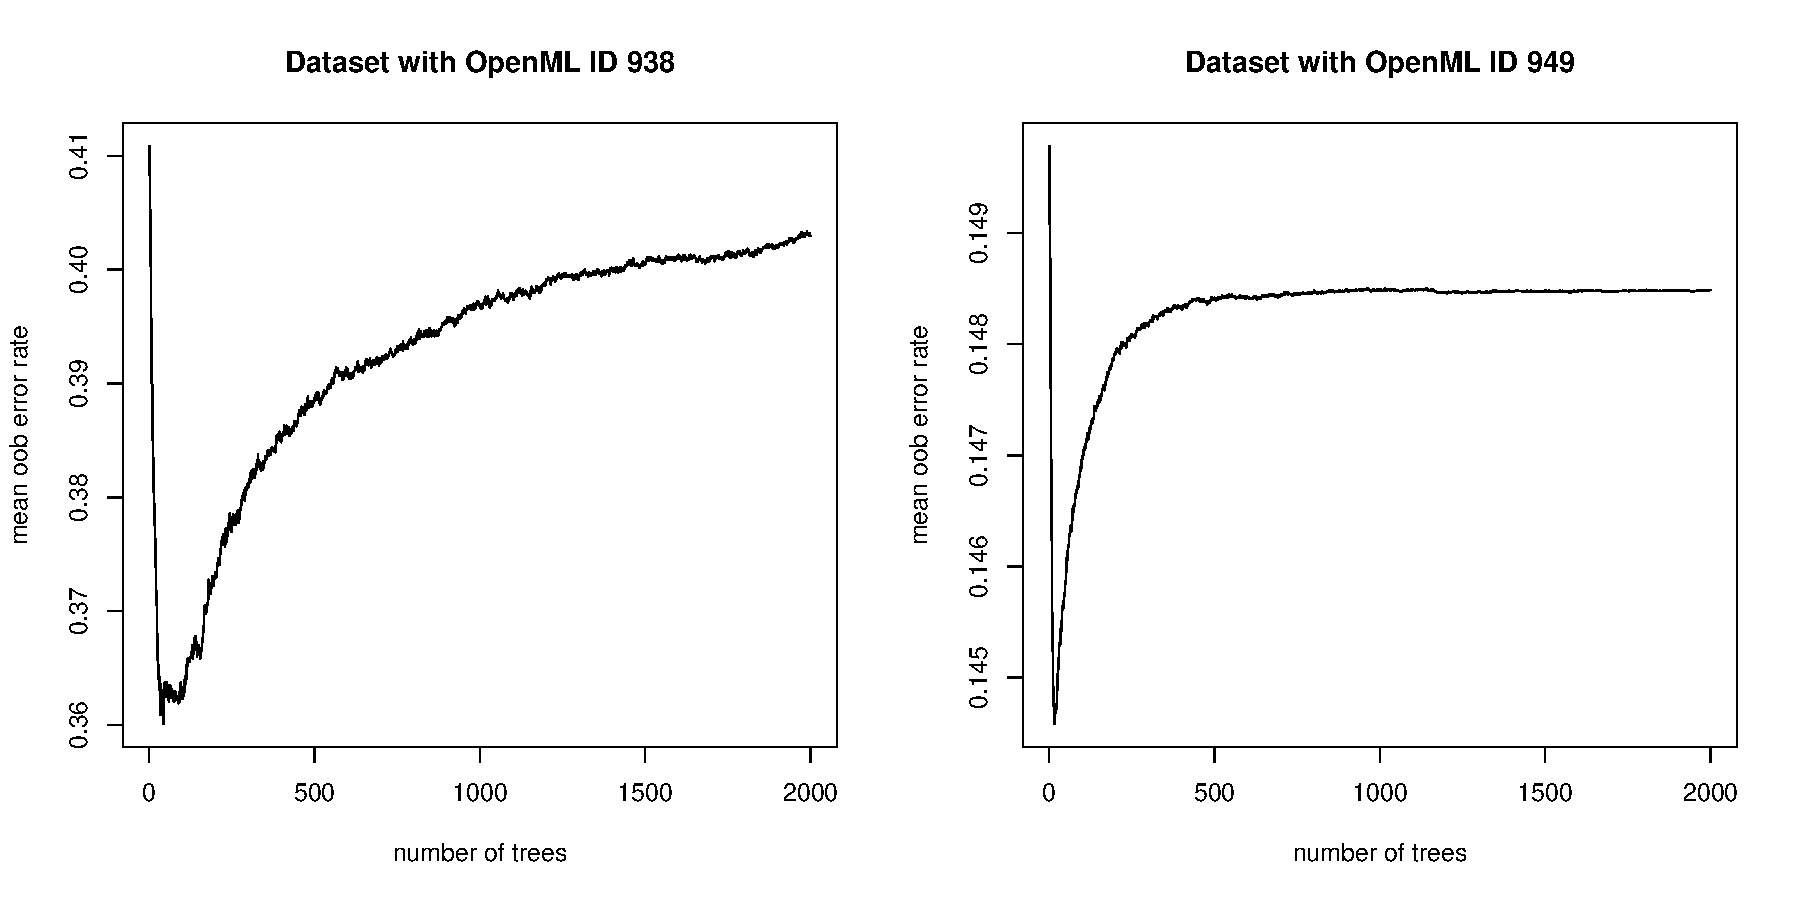
\includegraphics[width=\textwidth]{initial_example.pdf}
  \caption{Mean of OOB error curves of 1000 random forests}
   \label{fig:2examples}
\end{center}
\end{figure}

At first view, such non-monotonous patterns are a clear argument in favor of tuning  $T$. We claim, however, that it is important to understand why and in which circumstances such patterns happen in order to decide 
whether or not $T$ should be tuned in general. In Section \ref{sec:theory}, we address this issue from a theoretical point of view, by formulating the expected error rate as a function of the probabilities $\varepsilon_i$ 
of correct classification by a single tree for each observation $i$ of the training dataset, for $i=1,\dots,n$ (with $n$ denoting the size of the training dataset). This theoretical view provides a clear explanation of the 
non-monotonous error curve patterns. With a similar approach, we show that such non-monotonous patterns cannot be obtained with the Brier score or the logarithmic loss as accuracy measures which are based on probability estimations as well as with the mean squared 
error in the case of regression.

The rest of this paper is structured as follows. Section \ref{sec:background} is a brief introduction into random forest and error estimation. Theoretical results are presented in Section \ref{sec:theory}, while the 
results of a large empirical study based on XXX datasets from public database OpenML \citep{OpenML2013} are reported in Section \ref{sec:empirical}. More precisely, we empirically validate our theoretical model for the 
error as a function of the trees as well as our statements regarding the properties of datasets yielding non-monotonous patters. We finally argue in Section \ref{sec:discussion} that there is no inconvenience---except 
additional computational cost---in adding trees to a random forest and that  $T$  should thus not be seen as a tuning parameter. 



\section{Background: random forest and measures of accuracy}
\label{sec:background}
\subsection{Random forest}
The random forest (RF) is an ensemble learning technique consisting of the aggregation of a large number $T$ of decision trees, resulting in a reduction of variance compared to the single decision trees. 
In this paper we consider the original version of RF first described by \citep{Breiman2001}, while acknowledging that other variants exist, for example RF based on conditional inference trees \citep{Hothorn2006} 
which address the problem of variable selection bias investigated by \citet{Strobl2007}, extremely randomized trees \citep{Geurts2006} or ensembles of optimal trees \citet{Khan2016}. Our considerations are 
however generalizable to many of the available RF variants.

Each tree of the random forest is built based on a bootstrap sample (or a subsample) drawn randomly from the original training dataset using the CART method and the Gini impurity 
\citep{Breiman1984} as the splitting criterion. During the building of each tree of the forest, at each split, only a given number of candidate variables are considered. 
Random forest is considered a black-box algorithm, as gaining insight on a RF prediction rule is hard due to the large number of trees. One of the most common approaches to extract from 
the random forest interpretable information on the contribution of the different variables consists in the computation of the so-called variable importance measures. 

A prediction is obtained for a new observation by aggregating the predictions made by the $T$ single trees. In the case of regression RF, the most straightforward and common procedure 
consists of averaging the prediction of the single trees, while majority voting is usually applied to aggregate classification trees meaning that the new observation is assigned to the 
class that was most often predicted by the $T$ trees. 




%Another problem is the transportability of the random forest, as no convention exists on the implementation of the algorithm.

%\subsection{Out-of-bag error}
%The out-of-bag error is calculated by using the OOB estimations for the training observations. OOB estimations are calculated by predicting the class or probability for each training observation by 
%using only the trees, for which the observation was not used. These estimations are compared to the real values by calculating some performance measure like e.g. the mean missclassification error 
%which is the empirical counterpart of the generalization error. 

%To obtain more stable results and better estimations for the generalization error we repeated this procedure 100 times and averaged them. 

While RF can be used for various types of response variables including censored survival times or multicategorical variables, in this paper we focus on the two most common cases, regression and binary classification.

\subsection{General notations}
From now on, we consider a fixed training dataset $D$ consisting of $n$ observations, which is used to derive prediction rules by applying the RF algorithm with a number $T$ of trees.
Ideally, the performance of these prediction rules is estimated based on an independent test dataset, denoted as $D_{test}$, consisting of $n_{test}$ test observations.

Considering the $i$th observation from the test dataset ($i=1,\dots,n_{test}$), we denote its true response as $y_i$, which can be either a numeric value (in the case of regression) or the binary label 0 vs. 1 (in the case of binary classification).
The predicted value output by tree $t$ (with $t=1,\dots,T$) is denoted as $\hat{y}_{it}$, while $\hat{y}_i$ stands for the predicted value output by the whole random forest. Note that, in the case of regression, $\hat{y}_i$ is usually obtained by averaging as 
\[
\hat{y}_i=\frac{1}{T}\sum_{t=1}^T\hat{y}_{it}.
\]
In the case of classification, $\hat{y}_i$ is usually obtained by majority voting with a threshold of 0.5. For binary classification, it is equivalent to computing the same average as for regression, which now takes the form
\[
\hat{p}_i=\frac{1}{T}\sum_{t=1}^TI ( \hat{y}_{it}=1 )
\] 
and is denoted as $\hat{p}_i$ (standing for probability), and finally deriving $\hat{y}_i$ as
\[
   \hat{y}_{i} =
   \begin{cases}     1 & \text{if }\hat{p}_i>0.5,  \\
     0 & \text{otherwise.}
   \end{cases}
\]


\subsection{Measures of prediction error}
\label{subsec:errormeasures}
In regression as well as in classification, the prediction error of an RF for observation $i$ is usually quantified through a so-called loss function measuring the discrepancy between the true response $y_i$ and the predicted response $\hat{y}_i$ or, in the case of classification, between $y_i$ and $\hat{p}_i$. 

For both regression and binary classification, the classical and most straightforward error measure is defined for observation $i$ as 
\[
e_{i}\ =\ (y_i-\hat{y}_{i})^2\ =\ L(y_i,\hat{y}_{i})
\]
with the loss function $L(x,y)=(x-y)^2$. In the case of regression this is simply the squared error, while for binary classification it simplifies to
\[
   e_{i} =
   \begin{cases}     1 & \text{if observation } i \text{ is classified correctly by the RF}  \\
     0 & \text{otherwise.}
   \end{cases}
\]

Similarly, one can also consider the prediction error of single trees, i.e. the discrepancy between $y_i$ and $\hat{y}_{it}$. We define $e_{it}$ as 
\[
e_{it}=L(y_i,\hat{y}_{it})=(y_i-\hat{y}_{it})^2
\]
and the mean error as
\[
\varepsilon_i = E(e_{it}),
\]
where the expectation is taken over the possible trees conditionally on $D$---a quantity we need to derive our theoretical results on the dependence of accuracy measures on the number of tree $T$. The term $\varepsilon_i$ can be interpreted as the difficulty to predict $y_i$ with single trees. 
In the case of binary classification, we have $(y_i-\hat{y}_{it})^2=|y_i-\hat{y}_{it}|$ and $\varepsilon_i$ can be simply estimated as $|y_i-\hat{p}_i|$  from an RF with a large number of trees. 

In the case of binary classification, it is also common to quantify prediction error through the use of the Brier score, which has the form
\[
b_i\ =\ (y_i-\hat{p}_i)^2=L(y_i,\hat{p}_i)
\]
or of the logarithmic loss
\[
l_i\ =\ y_i\ln(\hat{p}_i)+(1-y_i)\ln (1-\hat{p}_i).
\]
Both of them are based on $\hat{p}_i$ rather than $\hat{y}_i$, and can thus be only defined for the whole RF and not for single trees.

\subsection{Test dataset vs. out-of-bag error}
In the cases where a test dataset $D_{test}$ is available, prediction error is assessed by summing the chosen error measure (as described in the previous paragraph) over the $n_{test}$ observations.

For example, for the classical error rate (for binary classification) and the mean squared error (for regression) are computed as
\[
\frac{1}{n_{test}}\sum_{i=1}^{n_{test}}(y-\hat{y}_i)^2.
\]

\section{Theoretical results}
\label{sec:theory}
In this section we compute the expected error---according to the different measures outlined in Section \ref{subsec:errormeasures}---of a RF consisting of $T$ trees as estimated based on the $n_{test}$ test observations, while considering the training dataset as fixed. The number $T$ of trees is considered a parameter of the RF and now mentioned in parentheses everytime we refer to the whole forest. In this section we are concerned with \textit{expected} errors, where expectation is taken over the sets of $T$ trees. Our goal is to study the monotonity of the expected errors with respect to $T$.


\subsection{Error rate (binary classification)}
\subsubsection{Theoretical considerations}
%so that $p_i := E(e_{it})$. $p_i$ can be estimated through the fraction of trees that missclassify $i$ for a big number of trees $T$. The error rate for the whole dataset for a random forest with $T$ trees and the typical threshold 0.5  for observation $i$
We first consider the classical error rate $e_i(T)$ for observation $i$ with an RF including $T$ trees and derive its expectation, conditional on the training set $D$. 
\begin{eqnarray*}
 E(e_i(T)) & = &  E \left(I \left( \left(\frac{1}{T} \sum_{t=1}^T e_{it} \right) > 0.5 \right) \right)\\
 & = & P \left( \left(\sum_{t=1}^T e_{it} \right) > 0.5 \cdot T \right). 
\end{eqnarray*}
We note that $e_{it}$ is a binary variable with $E(e_{it})=\varepsilon_i$ and that, the training dataset $D$ and the observation $i$ being fixed, the $e_{it}$ are mutually independent. It follows that  the sum $X_i=\sum_{t}^Te_{it}$ follows the binomial distribution $B(n, \varepsilon_i)$. 

It is immediate that the contribution of observation $i$ to the classical error, $P(X_i>0.5 \cdot T)$, is an increasing function in $T$ for $\varepsilon_i > 0.5$ and a decreasing function in $T$ for $\varepsilon_i < 0.5$. 

Note that in the above considerations we ignored the case where $\sum_{t=1}^T e_{it}  = 0.5 \cdot T$, which may happen in the case of an even $T$. In this case, the standard implementation in R (\texttt{randomForest}) assigns the observation randomly to a class. We choose to disregard this issue here as it will not change the results substantially (especially for large numbers of trees $T$) but would considerably complicate the formulas.  

\subsubsection{Impact on error curves}
Error curves for one observation with the mentioned adjustment in the case of odd number of trees and for different $\varepsilon_i$ can be seen in Figure \ref{fig:errorcurves}. Very high and very low numbers of $\varepsilon_i$ lead to rapid convergence, while for $\varepsilon_i$-values close to 0.5 more trees 
are needed to reach the plateau. 

\begin{figure}[!htb]
\begin{center}
  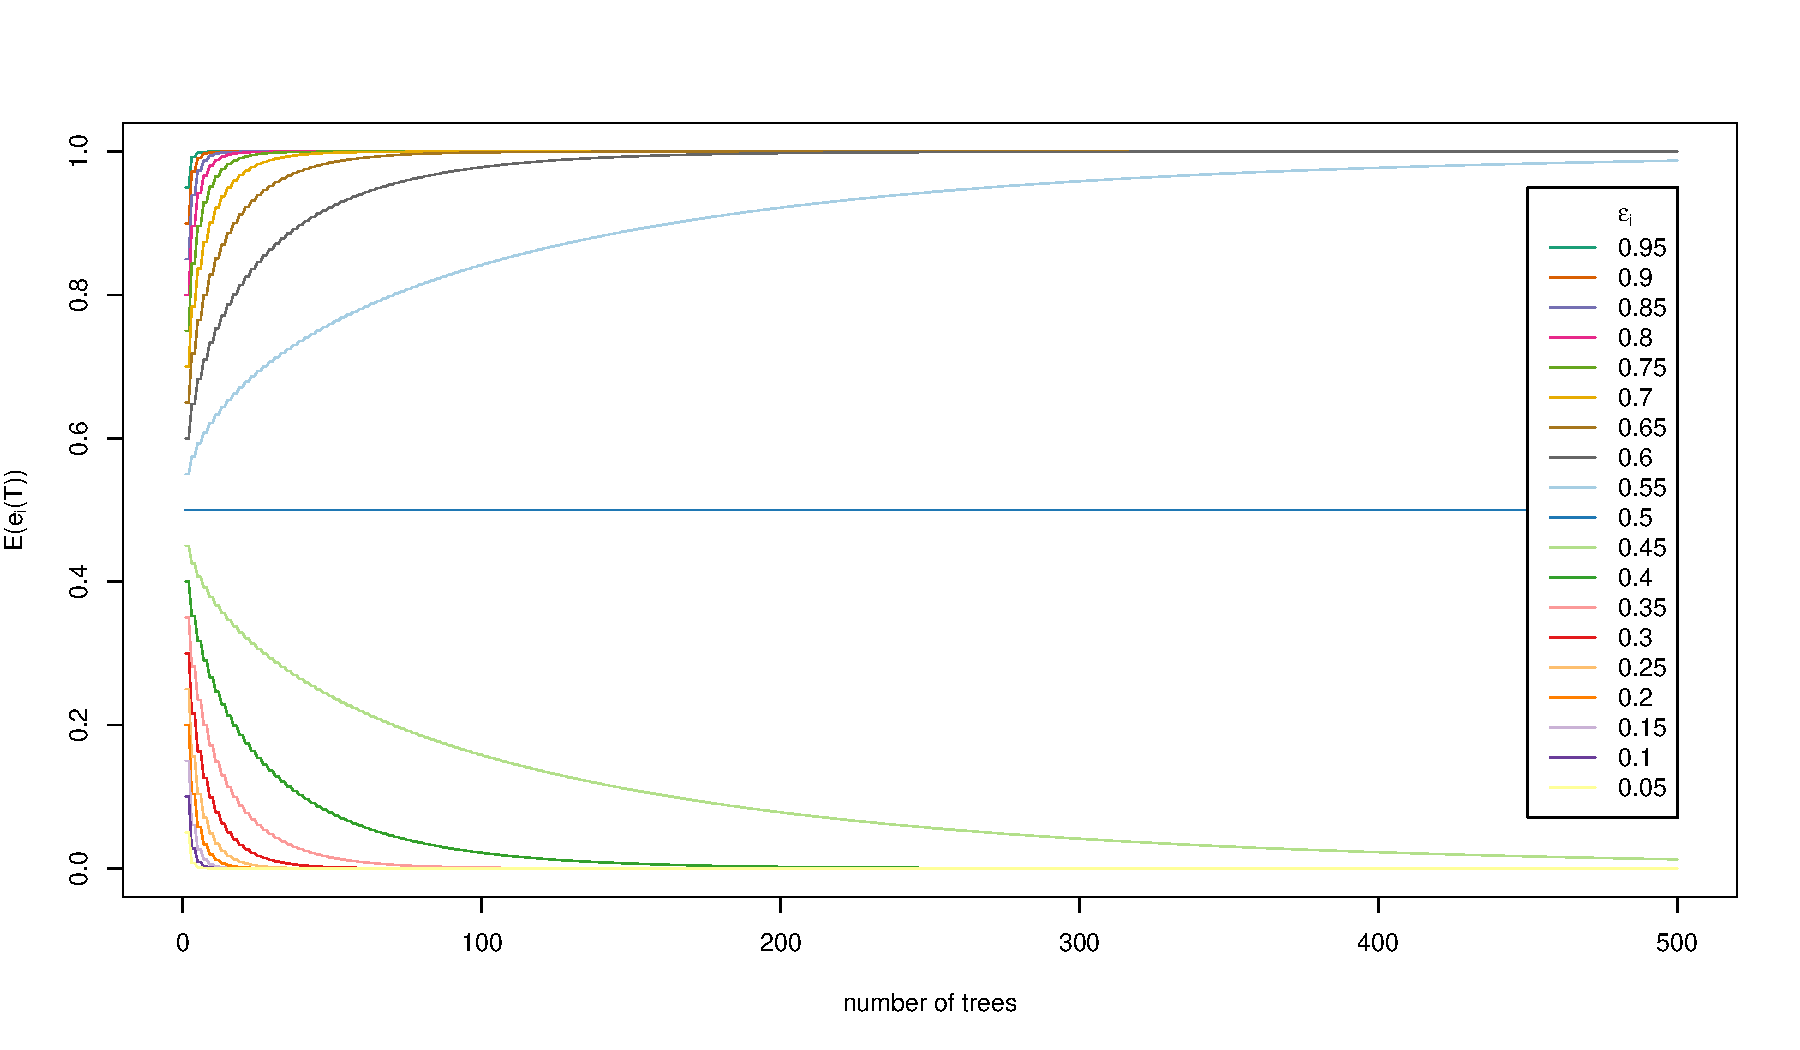
\includegraphics[width=\textwidth]{error_curves.pdf}
  \caption{Expected error for different $\varepsilon_i$ values}
  \label{fig:errorcurves}
\end{center}
\end{figure}

The error curve obtained for a test datasets consists of the average of the error curves of the single observations. Of course, if trees are good classifiers we should have $\varepsilon_i < 0.5$ for most observations. In many cases, observations with  $\varepsilon_i > 0.5$ will be compensated by observations with $\varepsilon_i < 0.5$ in such a way that the expected error curve is monotonously decreasing. This is typically the case if there are many observations with $\varepsilon_i\approx 0$ and a few with $\varepsilon\approx 1$.

However, if there are many observations with  $\varepsilon_i\approx 0$ and a few  observations with $\varepsilon_i \geq 0.5$ that are close to 0.5, the error curve first
falls down quickly because of the observation with $\varepsilon_i \approx 0$ and then grow again slowly as the number of trees increases because of the observations with $\varepsilon_i \geq 0.5$ close to 0.5. In Section \ref{sec:empirical}
we show that this is the case for the two examples depicted in the introduction. 

\subsubsection{Convergence speed of the error curve}
We see that the convergence of the error curve is only dependent on the distribution of the $\varepsilon_i$ of the observations. So the convergence speed of the error curve is not directly dependent 
on the number of observations $n$ or the number of features, but these characteristics could possibly influence the distribution and hence the convergence speed.  

In Section \ref{sec:empirical} we will try to look at typical distributions of the $\varepsilon_i$. We will also argue why it is better to look at Brier Score and AUC curves 
and propose a reasonable convergence stop criteria that takes that into account.




\subsection{Brier Score (binary classification) and squared error (regression)}
We now turn to the Brier score and compute the expected Brier score contribution of observation $i$ for a RF including $T$ trees, conditional on the training set $D$. We obtain
\begin{eqnarray*}
 E(b_i(T)) & = & E((y_i - \hat{p}_i(T) ) ^2) \\
                    & = & E \left( \left( y_i-\frac{1}{T}\sum_{t=1}^T\hat{y}_{it} \right)^2 \right) \\
                    & = & E \left( \left( \frac{1}{T}\sum_{t=1}^T(y_i-\hat{y}_{it}) \right)^2 \right) \\
                    & = & E \left( \left( \frac{1}{T}\sum_{t=1}^T e_{it} \right)^2 \right)
\end{eqnarray*} 


From $E(Z^2) = Var(Z)+E(Z)^2$ with $Z=\frac{1}{T}\sum_{t=1}^T e_{it}$  it follows:
\begin{eqnarray*}
 E(b_i(T)) & = & E(e_{it})^2+\frac{Var(e_{it})}{T},
\end{eqnarray*} 
which is obviously a strictly monotonous falling function of $T$. This also holds for the average over the observations of the test dataset. 

In the case of binary classification, we have  $e_{it}\sim\mathcal{B}(1,\varepsilon_i)$, yielding $E(e_{it})=\varepsilon_i$ and $Var(e_{it})=\varepsilon_i(1-\varepsilon_i)$, thus allowing the formulation of  $E(b_i(T))$ as $E(b_i(T))=\varepsilon_i^2+\frac{\varepsilon_i(1-\varepsilon_i)}{T}$.

The calculation is also valid for the squared error in the regression case, except that in this case we would write $\hat{y}_{i}$ instead of $\hat{p}_{i}$ in the first line. 

\subsection{Logarithmic Loss}
As outlined in Section \ref{subsec:errormeasures}, another usual error measure based on the discrepancy between $y_i$ and $\hat{p}_i$ is the logarithmic loss $l_i(T)=-(y_i\ln (\hat{p}_i(T))+(1-y_i)\ln (1-\hat{p}_i(T)))$. 
Noticing that $\hat{p}_i(T)=1-\frac{1}{T}\sum_{t=1}^Te_{it}$ for $y_i=1$ and $\hat{p}_i(T)=\frac{1}{T}\sum_{t=1}^Te_{it}$ for $y_i=0$, it can be in both cases $y_i=0$ and $y_i=1$ reformulated as
\[
l_i(T) =  -\ln \left( 1-\frac{1}{T}\sum_{t=1}^T e_{it} \right).
\]
We now use the Taylor expansion  (cite, e.g. Statistical theory with engineering applications, Hald, 1952)
\begin{align}
E\left[f(Z)\right]  {} = & E\left[f(\mu_Z + \left(Z - \mu_Z\right))\right] \nonumber \\
\approx & E \left[f(\mu_Z) + f'(\mu_Z)\left(Z-\mu_Z\right) + \frac{1}{2}f''(\mu_Z) \left(Z - \mu_Z\right)^2 \right] \nonumber \\
 = & f(E(Z)) + \frac{f''(E(Z))}{2} \cdot Var(Z) \nonumber
\end{align}
where $\mu_Z$ stands for $E(Z)$, $Z$ is defined as $Z=1-\frac{1}{T}\sum_{t=1}^T e_{it}$ and $f(.)$ as $f(.)=-\ln (.)$.
We have
\begin{eqnarray}
Var(Z) & = & \frac{\varepsilon_i(1-\varepsilon_i)}{T}\\
E(Z) & = & \varepsilon_i \\
f(E(Z)) & = & -\ln(\varepsilon_i) \\
f''(E(Z)) & = & \varepsilon_i^{-2},
\end{eqnarray}
finally yielding
\[
E(l_i(T)) \approx  -\ln (\varepsilon_i)+\frac{1-\varepsilon_i}{2T\varepsilon_i},
\]
which is obviously a decreasing function of $T$. Taylor approximation gets better and better for increasing $T$, since the variance of $l_i(T)$ decreases with increasing $T$ and $l_i(T)$ thus tends to get closer to its expectancy. Futhermore, note that we implicitly assumed that $\varepsilon_i\neq 0$. The case $\varepsilon_i=0$ is trivial, since we then always have $l_i(T)=0$, which does not depend on $T$.

\subsection{Adapting the models to the OOB error}
If there is no available test dataset, one can resort to the out-of-bag estimation technique, which uses only data from the training dataset $D$. The idea is to estimate, for each observation $i$ (for $i=1,\dots,n$) from the training dataset, the prediction error of the subforest consists of the trees for which this observation was not included in the bootstrap sample, i.e. was not used to construct the tree. Formally, the out-of-bag error is defined as
\[
OOB\ =\ \frac{1}{n}\sum_{i=1}^n\frac{1}{\sum_{t}^TI(i\notin B_t)}\sum_{t:\ i\notin B_t}...,
\]
where $B_t$ denotes the set of indices of the observations that were used to construct tree $t$.Is it really necessary to give details on OOB?

If one considers the OOB error instead of the test error from an independent dataset, the formulas given in the previous subsections are not directly applicable.
Indeed, the sums over the trees involved in the formulas should not be built over $T$ trees but only over the subset of trees for which the considered observation is out-of-bag, i.e. over $\approx\exp (-T)$ on average.

\section{Empirical results}
\label{sec:empirical}

This section shows a large-scale empirical study based on 193 real datasets from a publicly available database. The goals of this study are to (i) validate our theoretical formula for the expected prediction error by comparing it to the observed prediction error; give an order of magnitude of the frequency of non-monotonous patterns in real data settings; (iii) empirically confirm our statement that observations with $\varepsilon_i$ close to 0.5 are responsible for non-monotonous patterns. 

\subsection{Study design}
We analyse the OOB error curve of 193 datasets downloaded from the OpenML platform \citep{OpenML2013} satisfying the following criteria: the datasets have a pre-defined task in OpenML (see \citet{OpenML2013} for details on the OpenML nomenclature), they include less than 1000 observations and less than 1000 features. Cleaning procedures such as the deletion of duplicated datasets are also applied to obtain a decent collection of datasets. 

For each dataset we run the RF algorithm with $T=2000$ 1000 times successively with different seeds using the R package \texttt{randomForest} \citep{Liaw2002} and extract the OOB error curve, which is automatically calculated by the package. 
We calculate the mean curve over the 1000 runs by simple averaging. HOW MANY TREES?

\subsection{Overall results}
The graphs obtained for the 193 datasets can be seen in the supplementary material XXX. 
We observe that for most datasets the curve is quickly falling down until it converges to a dataset-specific plateau value. In about $10\%$ of the datasets, however, the curve is growing again after reaching its lowest value, leading to a value at 2000 trees that is by at least 0.005 bigger than the lowest value. Moreover, on very few datasets (3.6 \%) the curve is growing (almost) from the beginning, with the lowest value obtained for $\leq$20 trees. This odd pattern is observed mainly for smaller datasets: from the 7 datasets where this occurs 6 belong are the (RATHER THAN BELONG TO?) smallest datasets with respect to the product between number of observations and number of features. 

Importantly, we apply the theoretical model derived in Section \ref{subsec:errormeasures} to the 193 datasets. For each dataset, we compute the estimates $\hat{\varepsilon}_i=|y_i-\hat{p}_i|$  of the observation-specific errors $\varepsilon_i$ (as defined in Section \ref{subsec:errormeasures}) from an RF with a huge number $T=100000$: the more trees, the more accurate the estimates. Once the estimates $\hat{\varepsilon}_i=|y_i-\hat{p}_i|$ are computed, the curves of the $n$ observations can be derived and averaged to obtain the theoretical curve for the considered dataset.
It can be seen from the supplemental file (red curves), that our model fits the empirical curves very well.


\subsection{Datasets with non-monotonous curve}
We now examine in more detail the datasets yielding non-monotonous patterns. In particular, the histograms of the estimates $\hat{\varepsilon}_i=|y_i-\hat{p}_i|$ of the observation-specific errors $\varepsilon_i$  are of interest, since our theoretical results indicate that their distribution is crucial to the form of the error curve. 

Representative examples of histograms in the case of non-monotonous error rate can be seen in Figure XXX. The histograms belong to the datasets with OpenML ID 938 and 949 for which the OOB error curve was already depicted in the introduction in Figure \ref{fig:2examples}. 
For dataset 111 we included the histogram of values that where between 0.1 and 0.9 to see the relevant probabilities. In both cases we see, that we have a bigger amount of observations, that have a probability that is a bit smaller than 0.5
of being correctly classified than a bit bigger than 0.5 and hence concording with our theoretical results it follows that with growing number of trees these only nearly correctly classified observations will be wrongly classified and hence 
increase the error rate when enough trees are added to the ensemble. 

\begin{figure}[!htb]
\begin{center}
  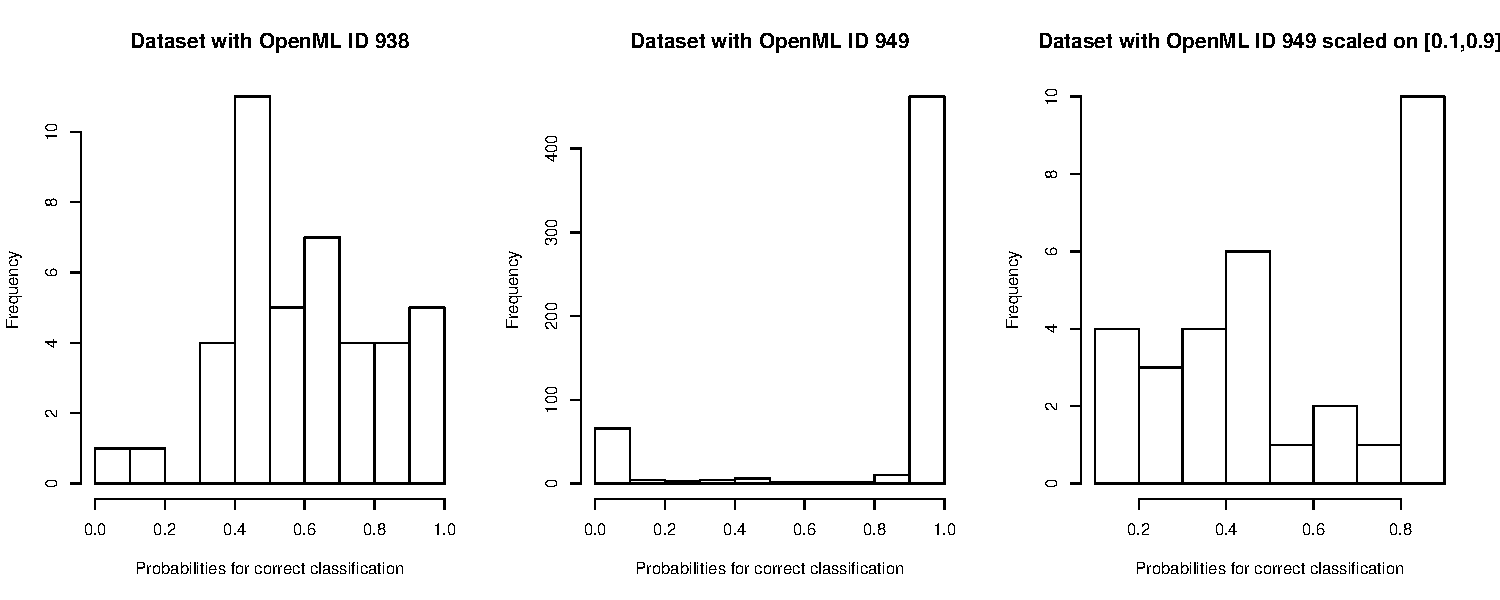
\includegraphics[width=\textwidth]{histogram.pdf}
  \caption{Histogram of the probability estimation of a random forest with 100000 trees}
\end{center}
\end{figure}


\section{Stopping criteria, AUC curves and Brier Score curves}
Automatic break criteria, convergence measure; (Question: Are more trees needed for bigger p/n to reach convergence? (Stackoverflow question: \url{http://stats.stackexchange.com/questions/243645/maximum-tree-needed-for-random-forest-modeling})

After x trees we reach a plateau in the AUC/Brier score curves...

Argue why more trees are nonetheless better: 
\begin{itemize}
\item Distribution of the probabilities of new observations do not necessarily have the patterns of the test (or OOB) observations. 
More likely, if the feature provide any useful information they will be rather correctly predicted with $\epsilon_i < 0.5$ than with $\epsilon_i > 0.5$ and hence more trees should be better. 
\item Measures like the brier score, logarithmic loss (and auc) provide more information about the predictions than the error rate.
\end{itemize}


\section{Recommendations and discussion}
\label{sec:discussion}

\begin{itemize}
 \item Generalization on any other bagging method (also with random samples of variables)
 \item Connection to the generalization error as described in Breiman
 \item Tune AUC for getting better MMCE (there was a paper about that)
 \item influence (theoretical) of sampsize and tree depth (see stackoverflow post: \url{http://stackoverflow.com/questions/34997134/random-forest-tuning-tree-depth-and-number-of-trees})
 \item Multiclass?
 \item Miscellaneous: oob error rate can be used for tuning, small differences between different R-packages (e.g. show different oob-plots or aggregation scheme (randomForest: predictions, party: proportion in leaves))
\end{itemize}

\section{Conclusion}

%\begin{figure}[!htb]
%\begin{center}
%\includegraphics[width=\textwidth]{baujahr2.eps}
%\caption{Relative Häufigkeit der Anzahl an gebauten Geräten sowie der Anzahl an Geräten, für die in 2014 mindestens ein Logbuch bzw. ein Help Ticket vorliegt}
%\end{center}
%\end{figure}
\bibliography{Ntree_RandomForest}

\end{document}

%\bibliography{Ntree_RandomForest}